\documentclass[10pt]{standalone}
\usepackage[utf8]{inputenc}
\usepackage{pgf,tikz,pgfplots}
\pgfplotsset{compat=1.15}
\usepackage{mathrsfs}
\usetikzlibrary{arrows}
\pagestyle{empty}
\begin{document}

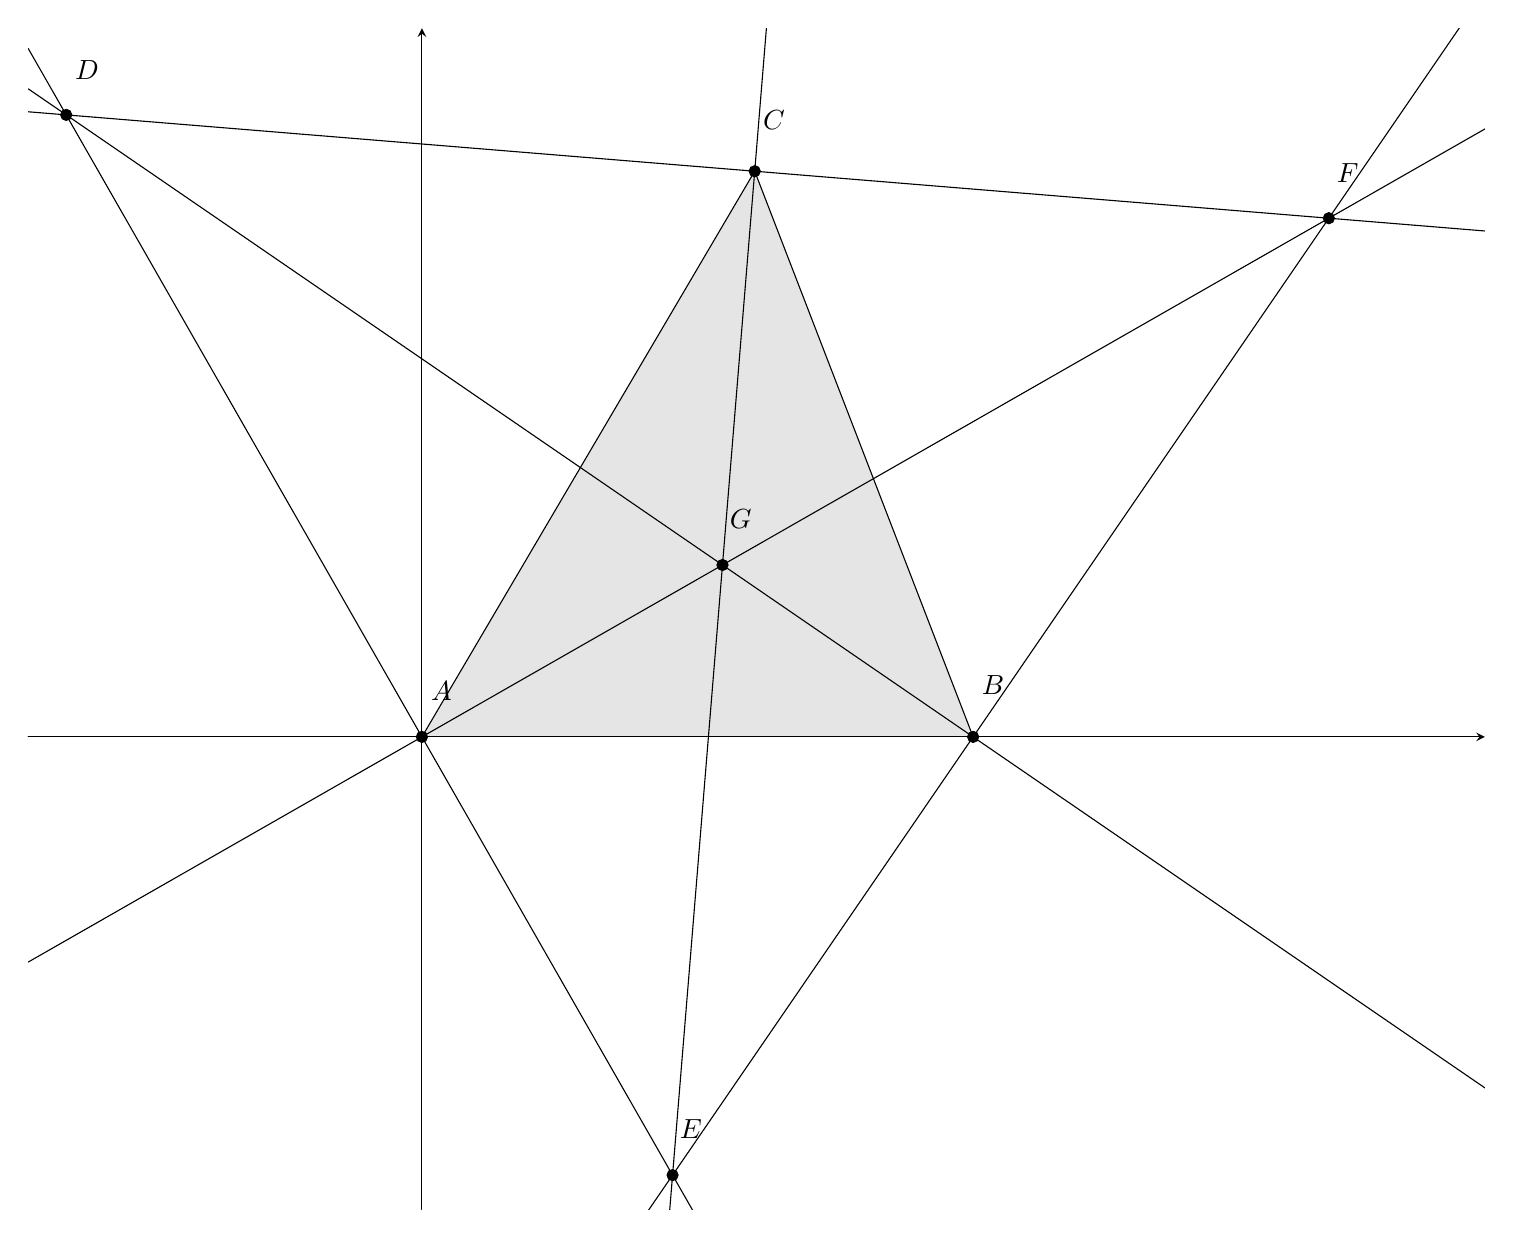
\begin{tikzpicture}[line cap=round,line join=round,>=triangle 45,x=1.0cm,y=1.0cm]
\begin{axis}[
x=1.0cm,y=1.0cm,
axis lines=middle,
xmin=-5.0,
xmax=13.5,
ymin=-6.0,
ymax=9.0,
ticks=none,]
\clip(-5.,-6.) rectangle (13.5,9.);
\fill[fill=black,fill opacity=0.1] (0.,0.) -- (7.,0.) -- (4.226204810235532,7.183752003695065) -- cycle;
\draw  (0.,0.)-- (7.,0.);
\draw  (7.,0.)-- (4.226204810235532,7.183752003695065);
\draw  (4.226204810235532,7.183752003695065)-- (0.,0.);
\draw [domain=-5.:13.5] plot(\x,{(-0.-0.8680615969584151*\x)/0.49645650754724296});
\draw [domain=-5.:13.5] plot(\x,{(-0.--0.49645650754724296*\x)/0.8680615969584151});
\draw [domain=-5.:13.5] plot(\x,{(-5.772776669005928--0.8246823812865612*\x)/0.5655961191482194});
\draw [domain=-5.:13.5] plot(\x,{(-3.9591728340375356--0.5655961191482194*\x)/-0.8246823812865612});
\draw [domain=-5.:13.5] plot(\x,{(-7.504483873118455--0.08155333557201537*\x)/-0.9966689788776805});
\draw [domain=-5.:13.5] plot(\x,{(--3.6262682949219074-0.9966689788776805*\x)/-0.08155333557201537});
\begin{scriptsize}
\draw [fill=black] (0.,0.) circle (2.0pt);
\draw (0.24944409814134996,0.5851446274325997) node {$A$};
\draw [fill=black] (7.,0.) circle (2.0pt);
\draw (7.252766060147918,0.6555297727793993) node {$B$};
\draw [fill=black] (4.226204810235532,7.183752003695065) circle (2.0pt);
\draw (4.472552818949331,7.8348145981529616) node {$C$};
\draw [fill=black] (-4.517678489481885,7.899228118691028) circle (2.0pt);
\draw (-4.25520520405383,8.468280906274158) node {$D$};
\draw [fill=black] (3.1829859367448132,-5.565498313231292) circle (2.0pt);
\draw (3.416775638747336,-4.97528185496457) node {$E$};
\draw [fill=black] (11.517678489481884,6.587120612149493) circle (2.0pt);
\draw (11.757415362343098,7.166155717358365) node {$F$};
\draw [fill=black] (3.817014063255187,2.1830034616692773) circle (2.0pt);
\draw (4.050241946868533,2.767084133183388) node {$G$};
\end{scriptsize}
\end{axis}
\end{tikzpicture}
\end{document}